\chapter{Evaluation}

This chapter covers the evaluation of the final product, the process model and what the team learned in this course.

\section{Challenges}
During the project several challenges were encountered. This section focuses on the two biggest of these challenges, licensing and the STK500 protocol.

	\subsection{Licensing}
	None of the group members had any experience with licensing prior to this project. The customer advised the group to use as much open source material as possible. All relevant open source systems deemed useful were incompatible with the Apache 2.0 licence, as they were licensed with GPL. Therefore it was necessary to implement the required functionality as part of the project. Initially the protocol was not a part of the assignment, but proved to be the most time consuming task of the project. \\

	As there were insecurities regarding whether implementations of the STK500 protocol could be licensed outside of GPL, it had to be implemented as a library. Repeated attempts to get the matter clarified by Atmel, the copyright holder of the STK500 protocol, were unsuccessful. \\

	\subsection{Protocol}\label{sec:protocol-issues}
	There were several difficulties related to programming the Arduino. There were few existing solutions for programming it in general, and none for Android or Java. The official implementation was available in C, but in the incompatible GPL license.\\

	The existence of certain programs written in Java with the purpose of programming Arduinos, led the group into assuming one of these could be utilized, as the license was compatible. When the time came to make use of it, it was discovered to internally use AVRDUDE as well - an embedded version of the latter was available for several platforms.\\

	This realization came somewhat late in the process, see Iteration 4 in Chapter \ref{sec:Iteration4}. Following this and the emergency meeting with the customer, it was decided to implement the protocol for programming Arduinos. Unfortunately, the documentation for these was a bit confusing; the most detailed and professional protocol document turned out to describe version 2 of the protocol~\cite{AVR068}. Version 2 was incompatible with the bootloader installed on the Arduino by default (Optiboot v4.4 on Arduino Uno). This was also the version that was partially implemented before the protocol differences and lack of backwards compatibility was discovered.\\

	The incompatibility could have been discovered earlier, but testing of the protocol had to be postponed. This was due to a lack of available working serial communication libraries in Java for PC's compatible with the Arduino Uno USB interface. Therefore a simple Android I/O app was added for testing purposes. Even then, the reason for the failure to communicate with the Arduino was hard to pin down, until a second Arduino was wired up to echo back the information the pair received.\\

	Changing the bootloader to utilize version 2 of the protocol could not be done due to it being licensed under GPL. Some attempts were made at finding compiled bootloaders for the Uno, but did not bear fruit. Attempts at compiling bootloaders using version 2 for the chip failed due to unresolved dependencies in the bootloader projects discovered, like the Stk-Boot~\cite{StkBoot} and uOS-Embedded~\cite{uOS-Embedded}.\\

	The solution was to implement version 1 of the protocol, and write off most of the protocol work as waste (a bit less than a weeks work). Some of the work done on version 2 could be reused despite the protocols being radically different, however. The second version of the protocol has a standardized message format with checksums and static tokens inside the messages to aid in error discovery; this would have been beneficial for communicating over Bluetooth.\\

	It was known that Optiboot didn't make use of all the commands specified in the protocol document AVR061~\cite{AVR061}, but documentation on which commands were superfluous was lacking. Since Optiboot would simply report that everything is fine when encountering such a command, discovering which were implemented or not had to be done by trial and error or investigating the source. The latter is designed to be very compact to fit in the 512kB threshold, which, if exceeded, would make the bootloader occupy 1024kB.\\

	Communicating with the Arduino proved fairly straightforward, but dealing with false positives was an issue. The Arduino would report that writing took place successfully, but writing would, for example, occur only in partial sections of the memory areas requested. The only way erroneous writing could be discovered, was to afterwards use an external program to read the written memory to verify its content. \\

	These issues prolonged the development of the system by a considerable amount, and had a major impact on the project. Some of these issues could have been avoided by more careful initial investigation, while others would not have been apparent prior to implementing the protocol.

	\subsection{Hard reset}
	\label{hard-reset}
	Due the development of the protocol, there were major problems programming the device without errors and it was needed a way to reset the Arduino to recover the programming. A lot of research were done to find out how the Arduino could be reset without using the excisting soft reset (using the ComputerSerial library).\\
	
	The hard reset feature was intended to provide the final fall back; this would be the only way to automatically recover from serious communication problems during programming (the Optiboot boot loader only waits for so long before leaving programming mode). In the case of the device ceasing to communicate with the protocol, reprogramming the device from a computer will be required in the absence of a hard reset feature.\\
	

\section{Interaction with the customer}
	Regular meetings with the customer were scheduled every Friday throughout the project. These meetings were used to present status, progress and any problems that were encountered. In these meetings the customer was able to aid the group in decisions and give input on the prototypes of the product. Apart from these regular meetings, the communication with the customer was done by e-mail. If difficult problems were encountered, or difficult decisions had to be made, the group was always able to achieve help from the customer. Extraordinary meetings could be scheduled at short notice if needed, and the customer was willing to request help from external developers if the group requested it.

\section{Group interaction}
	It was decided to schedule three regular group meetings each week, in addition to the meeting with the customer every Friday. Among these, two were to be team orientation meetings, where the group could discuss progress and issues and make plans for the coming week. The third meeting was a working session where the group worked together the whole day.
	In addition to these regular meetings the group scheduled working sessions continuously. The guidelines for the project stated that each group member should work approximately 20 hours each week, which meant at least three full days of work per group member each week. As described in Chapter \ref{communication}, interaction outside group meetings was mainly done by e-mail or on Skype. In Table~\ref{table:workhours} the total work hours for the group on every iteration is listed. The reduction of hours in iteration 4 was due to the Easter holidays. \\
	\newline
	Regarding interaction between the group members, no major issues were encountered. All team members were minded to work at least the suggested amount of hours each week and deliver a finished product at delivery date. To prevent potential conflicts, rules and roles were established at an early stage of the project. By establishing this at the beginning of the project, the group might have avoided larger discussions and disagreements at a later stage. Based on this, it is believed that the preventive measures taken by the group in the initiation phase has played a major role in the avoidance of conflicts and disagreements throughout the project.

	\begin{table}[H]
	\caption{Iterations and time spent}
	\centering
	\label{table:workhours}
	\begin{tabular}{|l|l|}
		\hline
			{\bf Iteration} & {\bf Hours}\\
		\hline
			Iteration 1 (Week 6-7) & 186 hours\\
		\hline
			Iteration 2 (Week 8-9) & 257 hours\\
		\hline
			Iteration 3 (Week 10-11) & 233 hours\\
		\hline
			Iteration 4 (Week 12-13) & 129 hours\\
		\hline
			Iteration 5 (Week 14-15) & 195 hours\\
		\hline
			Iteration 6 (Week 16-17) & 248.5 hours\\
		\hline
			Iteration 7 (Week 18-19) & 438 hours\\
		\hline
	\end{tabular}
	\end{table}

	An associated chart diagram of the work hours is shown in Figure~\ref{fig:workhours}

	\begin{figure}[H]
	\centering
	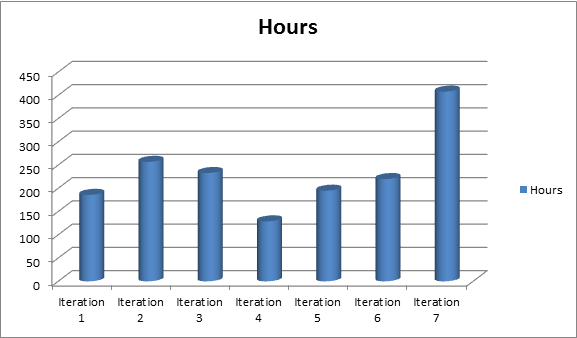
\includegraphics[scale=0.8]{images/workhours_chart2.png}
	\captionof{figure}{Work hours in each iteration throughout this project}
	\label{fig:workhours}
	\end{figure}

	\section{Lessons learned}
	This section describes the most important lessons learned by the group throughout the project. 

	\subsection{Prestudy}
	As mentioned in Section \ref{sec:protocol-issues}, it was originally assumed that an existing implementation of the STK500 protocol could be utilized. A more thorough prestudy would have revealed this assumption to be false at a considerably earlier stage. This would have allowed for more time to plan, implement, and test the implementation of the protocol. The lesson learned from this is to do a thorough prestudy early in the project, to back up every assumption with facts.

	\subsection{Project management}
	Based on the fact that every member of the group were used to different methods of communications during projects, the communication exceeded the expectations. This was because all members regularly checked Skype channel for messages. The lesson learned was that Skype proved to be an effective channel of communication within the group.\\

	As described in Chapter \ref{sec:GitHub} GitHub was used for version control. It is also possible to create issues highlighting what needs to be done within a project. These issues can be assigned to people, given labels to describe the issue, and be grouped to create a milestone. At times errors that should have been spotted have been merged into the master branch, introducing these errors to the master branch. These errors can be difficult to notice after the merging. An example of this is creating new features based on erroneous foundations. Based on this, future projects should meet test requirements before being merged into the master branch. \\

	\subsection{Design and Implementation}
	As described in Chapter \ref{sec:design-guide}, a complete design guide for the Android application was created early in the project. This guide proved to be very useful once the implementation began, as discussions on the design were avoided. Based on this, the group has learned that thorough planning of implementation is wise, as it increases the speed of the process and improves the quality of the final product.

	\subsection{Testing}
	Debugging the implementation of the STK500v1 protocol proved to be gruelling work. As described in Chapter \ref{sec:changes-desc}, testing was less prioritized than the implementation. As none of the group members had significant experience on the field, the writing of tests could potentially demand a lot of time that was used on other tasks. In hindsight, continuously writing tests for each new module in both the Android application and the protocol implementation, might have saved the group a lot of time spent on debugging.

	\section{Conclusion}
	The most important requirements were met. Those requirements not met were less prioritized after discussions with the customer. The project management methods applied, ensured steady progress throughout the project. The developer team considered the project to be successful as the single most important goal was attained: over-the-air installation.
